\chapter{Implementación}

La implementación del software se ha dividido en hitos. Estos, han sido definidos en Github
y cada uno de ellos contiene un grupo de \textit{issues} que se corresponden con las distintas
mejoras que ha ido incorporando el software a lo largo de su desarrollo.\\

Los hitos han sido los siguientes en orden cronológico:

\begin{enumerate}
	\item \textbf{Permitir registros y acceso de usuarios.}
	\item \textbf{Desarrollo del sistema de documentación.}
	\item \textbf{Desarrollo del sistema de croquis.}
	\item \textbf{Desarrollo del sistema de tests unitarios.}
	\item \textbf{Integración continua.}
	\item \textbf{Instalación de la aplicación de manera automática.}
\end{enumerate}

Toda la información relacionada con la implementación y el desarrollo se pueden encontrar en:

\begin{itemize}
	\item \href{https://github.com/Cerv1/Chief/milestones}{Lista de hitos.}
	\item \href{https://github.com/Cerv1/Chief/commits}{Lista de commits.}
\end{itemize}

\newpage

\section{Registro y acceso de usuarios.}
El objetivo de este hito es permitir que un usuario agente cree una cuenta en la aplicación 
y posteriormente pueda acceder a la misma si la contraseña y el usuario es válido. \\

Para poder utilizar el servidor de una manera más cómoda y con un mayor número de funcionalidades se ha utilizado
\textbf{Express.js}\cite{express} para crear el servicio web que se ofrece. De esta manera, conseguimos utilizar el 
servidor de una manera más eficiente.\\

Express.js ofrece un software liviano que dota de funcionalidades como negociación de contenido, una mejora en el 
rendimiento del servidor, la posibilidad de seleccionar un motor de plantillas para servir el contenido... En este caso,
se ha configurado para que utilice como motor de plantillas el ya mencionado \textbf{Pug}. De esta manera, cuando el usuario
realice una petición sobre alguna ruta se renderizará dicha plantilla para que el usuario reciba el archivo HTML, el cual
será interpretado por el navegador que esté utilizando.\\ 

Un usuario que quiera acceder a la aplicación o a cualquiera de las funcionalidades que ofrece deberá estar autenticado.
Para administrar de una manera más segura los datos de sesión de un usuario se ha utilizado la librería \textbf{Passport.js}\cite{passport}.
Esta librería se encarga de autenticar las peticiones hacia el servidor a través de una serie de \textit{plugins} conocidos
como \textit{strategies}. Gracias al comportamiento de esta librería podemos gestionar de una manera sencilla el acceso a los usuarios.
En este caso, se ha establecido un inicio de sesión mediante \textbf{usuario} y \textbf{contraseña} definidos por el agente en el 
momento de registrarse.\\

Cuando un agente realiza un registro, sus datos se almacenan \textbf{encriptados} en la base de datos para que de ninguna manera
se puedan alterar o recuperar de forma fraudulenta. El cifrado de dichos datos se realizan con un algoritmo basado en el cifrado
Blowfish\cite{blowfish} al que se le añaden unos bits aleatorios para proteger nuestro cifrado ante un ataque de Tabla Arcoíris\cite{rainbow}.


\section{Desarrollo del sistema de documentación.}

El primer objetivo de este hito es conseguir un sistema de incidencias completamente funcional y la posibiidad de generar todos los documentos
soportados por la plataforma de manera interactiva y desde cualquier localización. De esta manera se consigue que los agentes aumenten su 
productividad ya que pueden rellenar los documentos de manera inmediata y no tendrán que realizarlo al final del turno.\\

Para la realización de este hito se ha utilizado un módulo completamente propio llamado \textbf{doc\textunderscore functions}. Este módulo ha sido diseñado para ser usado
como biblioteca externa ya que contiene un gran número de funciones para generar los distintos tipos de documentos que podrá manejar la aplicación. De esta manera
se consigue una mejor reutilización del código, además de lograr un menor acoplamiento.\\

Esta biblioteca se encarga de crear el dato de tipo JSON que será posteriormente inyectado en las plantillas. Para ello, tiene en cuenta los datos recibidos
del servidor y otros que gestiona de manera independiente al usuario como pueden ser la fecha, la hora en la que se crea el turno, el formato de salida del 
documento... Además tiene otra función importante y es la de dar feedback al usuario. En la función en la que crea el documento se he creado un \textit{callback}
para poder comunicarse de nuevo con el servidor. De este modo, se podrá saber si la creación del documento ha sido correcta o, por el contrario, si ha fallado.
Podremos utilizar dicho \textit{callback} para devolver un \textit{feedback} al usuario y que sea consciente del resultado de la operación. Por tanto, todas las 
acciones de escritura y creación de documentos han sido desplazadas a dicho módulo, logrando así un mejor diseño y un código mejor estructurado.
\\

Una vez presentado el módulo creado para este hito, se procederá a detallar las funciones que se han creado para el usuario.

\subsection{Comienzo del turno de servicio.}
Cuando el agente desee comenzar un nuevo turno de servicio deberá introducir los datos relacionados con el mismo. Estos datos son los siguientes:

\begin{itemize}
	\item \textbf{Turno.} Podrá ser mañana, tarde o noche.
	\item \textbf{Identificadores de los policías.} Puede ser desde 1 hasta 4 los policías que estén en un turno simultáneamente.
	\item \textbf{Jefe de guardia.} El nombre del agente que actúa como supervisor del turno.
\end{itemize}

Una vez se rellenan estos campos, se creará un nuevo fichero de turno y se rellenarán las cabeceras con los datos anteriormente solicitados.

\subsection{Crear incidencias.}

En este caso, el agente podrá crear un nuevo registro perteneciente a una incidencia que será guardado en la base de datos. Para crear una nueva
incidencia se deberán rellenar los siguientes campos:

\begin{itemize}
	\item \textbf{Número de incidencia.} Número para identificarla. El agente decide que código le asigna.
	\item \textbf{Dependencia.} Dependencia desde la que se ha realizado la incidencia. Por ejemplo , alguien que llama por teléfono o una llamada de la central.
	\item \textbf{CEN.} Identificador del PREGUNTAR.
	\item \textbf{PP.LL.} Número del agente que registra la incidencia.
	\item \textbf{Hecho.} Descripción del motivo de la incidencia.
	\item \textbf{Actuación.} Acutación desempeñada por los agentes.
\end{itemize}

\subsection{Terminar el turno de servicio.}

Una vez terminado el servicio, se puede proceder a cerrar el parte de servicio. Cuando el agente realiza esta acción, \textbf{Chief} accede 
a la base de datos interna y genera un documento final. Este documento tendrá un nombre con el siguiente formato: \textit{DD\textunderscore MM\textunderscore YYYY\textunderscore Turno}.\\	

De esta manera, identificaremos a los partes de incidencias con un día, mes, año y nombre del turno. Es así debido a que no podrá haber más de un fichero de fin 
de turno para el mismo turno. Con este sistema se crean dichos documentos pero sin poder modificar las incidencias. Los registros que aparecen en el documento
final son todos los que han ocurrido dentro del intervalo del turno.

\subsection{Desarrollo del sistema de ordenanzas y accidentes.}

Una vez realizado el hito anterior, ya tenemos una aplicación con su sistema de identificación para los agentes y además pueden realizar todas las acciones
relacionadas con los partes de servicio habituales. Por tanto, faltaría incluir el sistema de accidentes y ordenanzas para completar el desarrollo de la
creación de documentos administrativos.\\

Todos los documentos serán generados en una carpeta específica donde serán agrupados todos los tipos de informes generados. En este caso, el nomrbe de los ficheros se
genera con el siguiente formato: \textit{DD\textunderscore MM\textunderscore YY\textunderscore HH:MM}.\\

Los documentos que el agente puede registrar son los siguientes:

\begin{itemize}
	\item \textbf{Ordenanza de limpieza. } Se generará un acta de denuncia ante la ordenanza de limpieza.
	\item \textbf{Ordenanza de ruidos en la vía pública. } Se generará un acta de denuncia por ruidos u otras actividades molestas en en la vía pública bajo el artículo número
	43.2, del Decreto 326/03 y la Ley 7/06 de 24 de Octubre. REFS NEEDED.
	\item \textbf{Ordenanza de ruidos en domicilio. } Se generará un acta de denuncia con el artículo elegido por el agente de la Ley 37/2003 y bajo el Decreto 326/03. REFS NEEDED.
	\item \textbf{Ordenanza de ruidos en local. }  Se generará un acta de denuncia con el artículo elegido por el agente de la Ley 37/2003 y bajo el Decreto 326/03. REFS NEEDED.
	\item \textbf{Acta de medición de ruidos. } Se generará un acta de medición de ruidos bajo el artículo elegido por el agente de la Ley 37/2003 y bajo el Decreto 326/03. REFS NEEDED.
	\item \textbf{Acta de inspección de obras. }  Se generará un acta de inspección de obras y quedará numerada bajo el número de acta elegido por el agente.
	\item \textbf{Acta de hallazgo de residuos. } Se generará un acta de denuncia en la que queda constancia de que se dará parte a la Concejalía de Medioambiente y Urbanismo
	\item \textbf{Accidente de 2 vehículos. } Se creará un diligencia en la que quedarán registrados los datos de todos los involucrados en el accidente, tanto testigos como 
	conductores de los vehículos.
	\item \textbf{Accidente de 3 vehículos. } Se creará un diligencia en la que quedarán registrados los datos de todos los involucrados en el accidente, tanto testigos como 
	conductores de los vehículos.
\end{itemize}

\section{Desarrollo del sistema de croquis.}

En esta etapa del desarrollo el agente ya dispone de un sistema de acceso y de documentación completa. Para este hito se piensa en la dificultad que tiene un agente para 
demostrar que los hechos han ocurrido tal y como se han registrado pasado un tiempo del incidente.\\

Por ejemplo, hay un accidente porque el \textit{vehículo A} no ha respetado un ceda el paso e impacta contra el \textit{vehículo B} generando ciertos desperfectos en ambos
vehículos. Los involucrados junto con los agentes realizan un parte en el que quedan constatados los daños.  Un tiempo después, hay una reclamación por parte de uno de los
involucrados debido a que su vehículo tiene más desperfectos de los que se apuntaron a causa del accidente y el seguro no se hace responsable de cubrir dichos desperfectos
debido a que en el parte no se menciona nada acerca de dichos daños. En este caso, es su palabra contra la del agente.\\

Para evitar estas situaciones se ha diseñado este sistema. El agente podrá tomar una fotografía de los hechos y dibujar sobre ella todo lo que quiera. Además, se 
pueden hacer anotaciones sobre la propia imagen para reflejar datos de importancia como la dirección en la que venían los vehículos, resaltar puntos de la imagen...\\

Una vez el agente ha realizado todas las fotografías pertinentes y con todo lujo de detalles para que no pueda ocurrir la situación previamente descrita,
puede proceder a enviarlas al servidor donde quedarán almacenadas para posteriores consultas. De este modo, aunque pase mucho tiempo, siempre se podrán recurrir a 
las fotografías de aquel momento con todas las anotaciones que se tomaron para situarse en un contexto lo más cercano posible al de la incidencia. \\

Para desarrollar esta funcionalidad se ha utilizado \textit{canvas}\cite{canvas}. Este tipo de elemento es muy potente debido a que está expresamente diseñado para 
dibujar gráficos en un entorno web utilizando JavaScript. Cabe destacar, que \textit{canvas} es \textbf{únicamente} un elemento que está preparado para contener gráficos.
Es decir, dichos gráficos los tenemos que insertar mediante el uso de JavaScript y no forman parte del elemento de forma nativa.\\

Para crear el croquis, el agente puede tomar una foto o subir una desde el almacenamiento interno. Una vez cargada la imagen, se mostrará en pantalla y se podrá 
dibujar sobre ella. Para lograr esta funcionalidad, se detecta cuando se ha subido una imagen a la aplicación y la inserta directamente en el canvas, sobre el que 
podremos dibujar y, además, borrar el contenido del croquis si es erróneo, o se quiere volver a comenzar.

\section{Tests unitarios.}

En este hito ya se dan por realizadas las funcionalidades que podrán usar los agentes. En este punto, nos centramos en probar la calidad del software y del diseño.
Para ello, se ha empleado un sistema de \textbf{test unitarios}.\\

Los test unitarios están realizados con el propósito de probar las funcionalidades de la aplicación y así poder evitar los posibles errores en nuestro código \textbf{antes}
del despliegue de la aplicación. Estos test se implementan de manera individual y el objetivo de cada uno de ellos es probar una funcionalidad. Para ello, se realizan varias
pruebas sobre la misma característica con distintas entradas y de las que conocemos los resultados que debieran ser correctos o erróneos. Un hecho relevante en la inclusión
de estos tests en nuestro sistema es que, además de garantizar el correcto funcionamiento de la aplicación antes de realizar el despliegue, es que pueden ser automatizados. 
De esta manera y con la ayuda de un sistema de integración continua que veremos en el siguiente punto, conseguimos que cada vez que se realice una modificación en nuestro software
se compruebe la integridad del sistema rehaciendo los tests.\\

\begin{figure}[H]
	\centering
	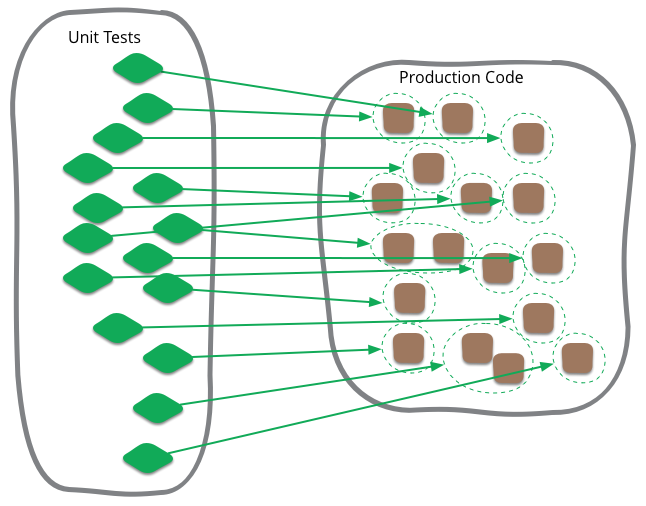
\includegraphics[scale=0.45]{imagenes/unit-test.png}
	\caption{Esquema del funcionamiento de los tests unitarios. \label{fig:figura13}}
\end{figure}

En este caso, se ha utilizado la librería \textit{supertest}\cite{supertest}, la cual nos proporciona un alto nivel de abstracción para probar nuestro servidor web.
Los test unitarios que se han realizado prueban las siguientes funcionalidades:

\begin{itemize}
	\item \textbf{Servidor.} Se realizan consultas a todas las rutas posibles de la aplicación para comprobar que todas existen y que además, solo se puede acceder 
	si se está previamente identificado. De este modo, garantizamos no solamente que todas las rutas posibles de la aplicación están operativas, sino que podemos garantizar
	que ningún usuario no identificado va a poder acceder a esta aplicación, consiguiendo probar parte de la seguridad de la aplicación antes del despliegue.
	\item \textbf{Base de datos.} Se realiza la creación de un usuario de prueba y se añade a la base de datos. Posteriormente, se comprueba si dicho usuario a quedado registrado
	en la base de datos y se procede a borrar para no ensuciar los registros. De igual manera se realiza con las incidencias, creando una de prueba y probando posteriormente que
	existe. Una vez realizado este test, se puede estar seguro de que la base de datos está configurada correctamente y completamente funcional.
\end{itemize}  

\section{Integración continua.}

Como objetivo de este hito, se propone añadir a nuestro desarrollo un sistema de integración continua.\\

La integración continua se creó con la intención de realizar el proceso de integración del software (ejecución de los tests) de la manera más habitual posible. De este modo, 
podemos detectar los fallos de manera inmediata y antes de que pase a la etapa de producción.\\

Para lograrlo se ha utilizado \textit{Travis CI}\cite{travis-ci}. Con esta herramienta es muy rápido y sencillo añadir la integración continua a nuestro repositorio. Para ello,
tan solo tenemos registrarnos en su página web con nuestra cuenta de GitHub, dar de alta el repositorio. Para que funcione correctamente, se debe crear un fichero de configuración
llamado \verb|.travis.yml|. Este archivo es el encargado de indicarle a \textit{Travis} el contexto en el que se ejecutarán los test, por tanto contiene
información relacionada con el lenguaje de programación utilizado, las versiones utilizadas, si se necesita permisos de superusuario...\\

En la siguiente imagen se representan los siguientes estados por los que pasa el código fuente desde que se añade hasta que ha pasado todos los test y la fase de integración.

\begin{figure}[H]
	\centering
	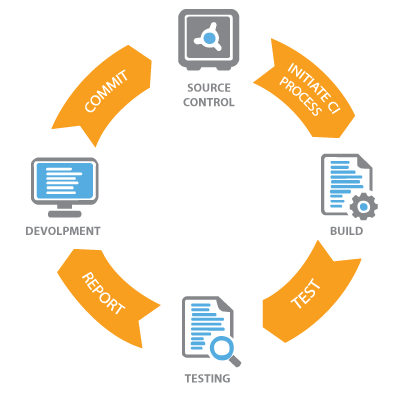
\includegraphics[scale=0.6]{imagenes/continuous-integration.png}
	\caption{Esquema del funcionamiento de un sistema de integración continua. \label{fig:figura14}}
\end{figure}

\section{Instalación de la aplicación de manera automática.}
Para finalizar el desarrollo, se ha configurado el entorno de tal manera que la aplicación se configure automáticamente y esté lista para desplegarse de manera rápida y clara.\\

Para conseguir dichos objetivos, se han utilizado dos herramientas presentadas en el previo análisis: \textit{Vagrant} y \textit{Ansible}. 

\subsection{Creación del entorno.}

La aplicación se ejecutará bajo una máquina virtual que corre con \textit{Ubuntu 16.04}. La elección de este sistema operativo ha sido por los siguientes motivos:
\begin{itemize}
	\item \textbf{Compatibilidad.} Aunque la aplicación será compatible con todos los navegadores del mercado, el servidor deberá estar basado en Linux. Además, 
	Ubuntu en la versión 16.04 es LTS(\textit{Long Term Support}), por lo tanto, es una buena opción para mantener una máquina virtual a largo plazo. Otro motivo para
	elegir este sistema operativo en concreto y no su versión \textit{Server} es debido a que \textit{Vagrant} no tiene una imagen oficial de dicho sistema. Por tanto,
	para evitar vulnerabilidades a largo plazo se ha optado por esta versión en concreto.
	
	\item \textbf{Uso.} Ubuntu es la distribución basada en Linux más usada del mundo\cite{ubuntu-usage} y por tanto tiene una amplia comunidad de desarrolladores. Esto
	hace que sea un sistema operativo muy estable en sus versiones \textit{LTS}, lo cual es ideal para nuestro servidor.
\end{itemize}

Una vez elegido el sistema operativo, \textit{Vagrant} realiza las siguientes operaciones:

\begin{itemize}
	\item \textbf{Instala el S.O.} Si no hay registro en la máquina local del S.O, lo descargará e instalará antes de comenzar.
	\item \textbf{Actualiza el S.O.} Comprueba la versión del sistema operativo en busca de nuevas actualizaciones antes de lanzar la máquina virtual.
	\item \textbf{Ajusta las claves ssh.} Utiliza un esquema de llave pública/privada y de este modo podremos acceder a la máquina virtual de manera segura y sin contraseña.
	\item \textbf{Redirecciona los puertos.} Configura los puertos que queramos redireccionar de nuestra máquina local a la virtual, consiguiendo desviar el tráfico 
	para ser atendido por nuestro servidor.
	\item \textbf{Provisiona.} Ejecuta \textit{Ansible} para provisionar a la máquina con los recursos necesarios.
\end{itemize}

Una vez se llega a este punto, \textit{Vagrant} ejecuta el \textit{Playbook} de \textit{Ansible}. Dicho fichero contiene las instrucciones necesarias para 
preparar la máquina con todas las dependencias que tenga nuestro proyecto. Esto se traduce directamente en que con este tipo de ficheros se puede automatizar acciones
como actualizar la lista de paquetes del sistema, descargar dependencias globales de la aplicación, instalar \textbf{Chief}, ejecutar los test, lanzar la aplicación...\\

